\documentclass[10pt]{article}         %% What type of document you're writing.

%%%%% Preamble

%% Packages to use

\usepackage{amsmath,amsfonts,amssymb}   %% AMS mathematics macros
\usepackage{graphicx}
\usepackage{lmodern}  % for bold teletype font
\usepackage{amsmath}  % for \hookrightarrow
\usepackage{xcolor}   % for \textcolor
\usepackage{listings}
\lstset{
  basicstyle=\ttfamily,
  columns=fullflexible,
  frame=single,
  breaklines=true,
  postbreak=\mbox{\textcolor{red}{$\hookrightarrow$}\space},
}

%% Title Information.

\title{HomeWork 04}
\author{Deep Dand}
%% \date{2 July 2004}           %% By default, LaTeX uses the current date

%%%%% The Document

\begin{document}

\maketitle

\begin{abstract}
KNN Regressor
\end{abstract}

\section{Problem}
\subsection{a}
You will modify the python code below to generate 1000 data points
The code below generates 1000 data points 

Code Begins
\lstinputlisting{hw4a.py}
Code ends
\\Output\\
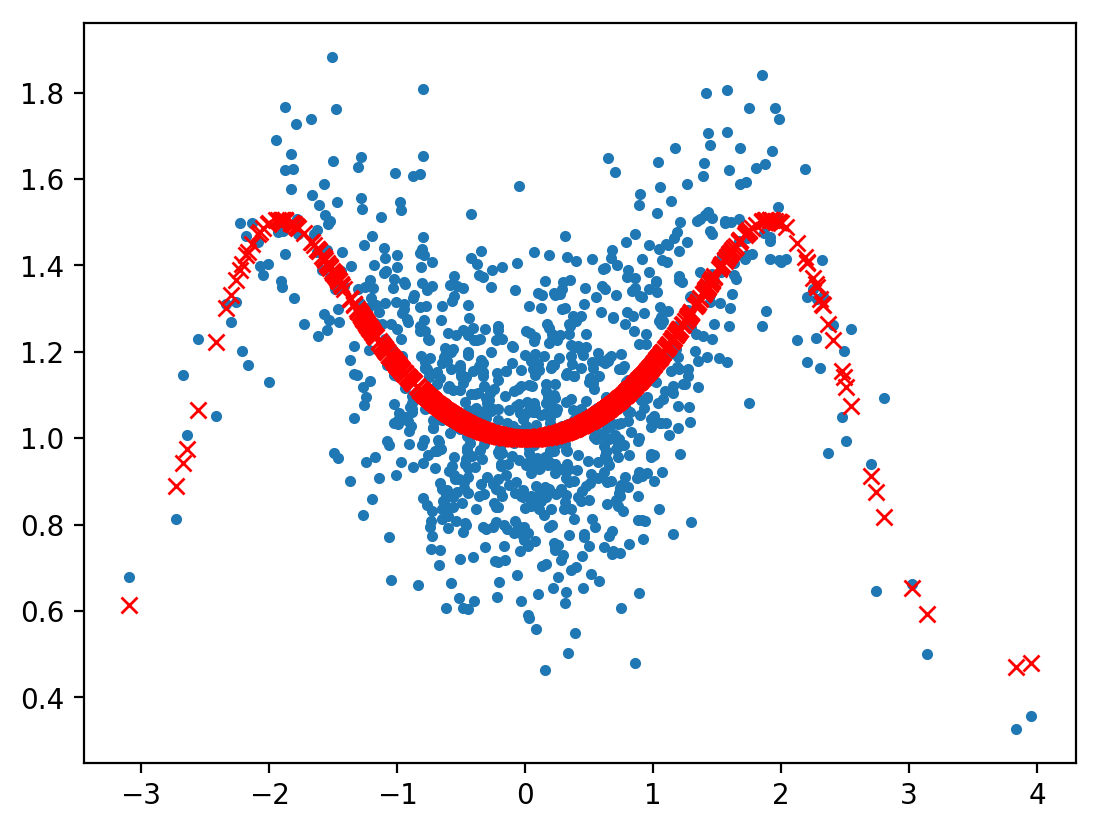
\includegraphics[scale=0.45]{HW4_PartA}

\\The pocket algorithm takes 15 iterations for the execution time and finds the best classification. The best weight is $$w = [8,  0.655, 2.6699]$$ and the best result came at iteration 15.
\subsection{b}
Using 10-fold CV, you will report the three best values of k-neighbors that yield the best CV
Eout. You will vary the values of k in the following range: k = 1; 3; 5;

\\You will report the best CV Eout.
Code Begins
\lstinputlisting{hw4btt.py}
Code ends. 
\\Output\\
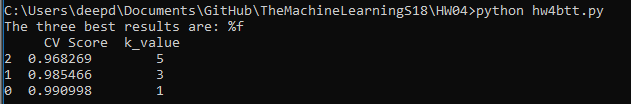
\includegraphics[scale=0.45]{hw4q1partc}
\\The linear regression takes only 1 iterations for the execution time and finds the best classification. The best weight is $$w = [0.1243,  0.2383, 0.0757]$$ and the best result came at iteration 1.

\end{document}

